%%「論文」,「レター」,「レター(C分冊)」,「技術研究報告」などのテンプレート
%% 1. 「論文」
%% v3.0 [2015/11/14]

\documentclass[paper]{ieicej}
%\documentclass[invited]{ieicej}% 招待論文
%\documentclass[survey]{ieicej}% サーベイ論文
%\documentclass[comment]{ieicej}% 解説論文



%\usepackage[dvips]{graphicx}
%\usepackage[dviout]{graphicx}
\usepackage[dvipdfmx]{graphicx,xcolor}
\usepackage[T1]{fontenc}
\usepackage{lmodern}
\usepackage{textcomp}
\usepackage{latexsym}
%\usepackage[fleqn]{amsmath}
%\usepackage{amssymb}

\setcounter{page}{1}

\field{}
\jtitle{開発標準プロセスを用いた不完全なソフトウェア要求に対する問題検出の分類法}
\etitle{}
\authorlist{%
 \authorentry{}{}{}\MembershipNumber{}
 %\authorentry{和文著者名}{英文著者名}{所属ラベル}\MembershipNumber{}
 %\authorentry[メールアドレス]{和文著者名}{英文著者名}{所属ラベル}\MembershipNumber{}
 %\authorentry{和文著者名}{英文著者名}{所属ラベル}[現在の所属ラベル]\MembershipNumber{}
}
\affiliate[]{}{}
%\affiliate[所属ラベル]{和文所属}{英文所属}
%\paffiliate[]{}
%\paffiliate[現在の所属ラベル]{和文所属}

\begin{document}
\begin{abstract}
%和文あらまし 500字以内
�F���@�̃\�t�g�E�F�A�ɂ����āA�\�t�g�E�F�A�̕s��̓~�b�V�����̐����ɑ΂��đ傫�ȖW���ƂȂ��Ă���B
�{�����ł̓\�t�g�E�F�A�s��̑傫�Ȍ����ƂȂ��Ă���v���R��ɒ��ڂ����B
���ۂɉF���@�Ŕ��������\�t�g�E�F�A�̕s������ɁA���ׂ̕��ނƊJ���W���v���Z�X�̂Q�‚̊ϓ_����s��̕��ނ��s���Ă���B
���̕��ނ��s�����ƂŁA�ǂ̂悤�ȕs��������̂��A�ǂ̃v���Z�X�ɂ����ĕs����������₷���̂������m�ɂȂ�B


\end{abstract}
\begin{keyword}
%和文キーワード 4〜5語
\end{keyword}
\begin{eabstract}
%英文アブストラクト 100 words
\end{eabstract}
\begin{ekeyword}
%英文キーワード
\end{ekeyword}
\maketitle

%%\section{まえがき}
\section{はじめに}
�V�X�e���J���̍ۂɁC�\�t�g�E�F�A�������Ŕ�������s��͑傫��2�p�^�[���ɕ����邱�Ƃ��ł���D
1�–ڂ�``���߂��Ă���v���͐��������C�\�t�g�E�F�A�̎���������Ă���''�p�^�[���ł���C2�–ڂ�``�����͗v���ʂ�ł��邪�C�v�����s���S�ł���''�p�^�[���ł���D
�O�҂̃\�t�g�E�F�A�̎����ɂ�������̓c�[���Ȃǂ�p���邱�ƂŔ����ł���D
����ŁC��҂Ɋւ��ẮC�c�[�������݂����C�v���d�l�����ɂ��L�ڂ���Ă��Ȃ����ߔ���������ł���D
�܂��C�\�t�g�E�F�A�̎����ɂ�����s��̊����͔��ɏ��Ȃ����Ƃ����������Ŗ��炩�ɂ��Ă���\cite{4812749}�D
����āC�\�t�g�E�F�A�̐M���������߂邽�߂ɂ́C�\�t�g�E�F�A�̎����ɂ��s������łȂ��C�v���R��ɂ��s��ɂ����Ă��l������K�v������D

Avizienis��́C�s��S�̗̂v����1�‚ł��錇�ׂɊւ��镪�ޖ@���Ă��Ă���\cite{1335465}�D
�������C�ÓI�Ȍ��ׂ̕��ނ����ł́C�ڍׂȌ�����Nj����邱�Ƃ��ł����C�v�����s���S�ł��鎖�ۂɑ΂��Ă͔���������ł���D
����Ė{�����ł́C���I�ł���J���H���i�v���Z�X�j�ɒ��ڂ��邱�ƂŁC�v�����s���S�ł��邱�Ƃɑ΂��āC�Ώ��􂪔����ł���ƍl�����D

�{�����ł́C�F���@�ƌĂ΂��C�l�H�q���⃍�P�b�g�ȂǂŎ��ۂɔ���������������ƂɁC���ׂ̕��ނƊJ���H���ł���v���Z�X��2�‚̊ϓ_����s��̕��ށE���͂��s�����D
���̕��͂ɂ��C�ΏۃV�X�e���ɂ����āC�ǂ̂悤�Ȍ��ׂɊ�Â��s��������̂��C�܂��قȂ�v���Z�X�ɂɂ����ĉe�����y�ڂ��Ă���̂͂ǂ�ł��邩�����m�ɂȂ�ƍl������D

�{�_���̍\�����ȉ��Ɏ����D
2�͂ł͌����̔w�i�ɂ‚��Đ������C3�͂Œ�Ă��镪�ނ̘g�g�݂ɂ‚��ďq�ׂ�D
4�͂ł͎��ۂɃf�[�^��K�p�������ʂ��q�ׁC5�͂ōl�@�C6�͂ł܂Ƃ߂⍡��̉ۑ�ɂ‚��ďq�ׂ�D


\section{背景}
�F���@�ƌĂ΂��A�l�H�q���⃍�P�b�g�Ȃǂ͈�x��΂��Ă��܂��Ɨe�ՂɏC�����ł��Ȃ��A���i���P���A�J�����Ԃ������A���‹��Ńe�X�g�ł��Ȃ��Ȃǂ̓���������\cite{JAXA2}\cite{JAXA3}�B
����āA�F���@�̃\�t�g�E�F�A�J���ɂ����āA�����Ɏ��s���Ȃ����̂ł��邩�A���Ȃ킿���M���������߂���͕̂K�v�s�Œ��ł��B
���M�����V�X�e���ł͏�Q�Ƃ��Č��������Ȃ��悤�ȑ΍􂪕K�v�ƂȂ�B
������������邽�߂ɁA�����̐ÓI�ȕ��ނ��s�Ă��錤�������ł͕s�\���ł���B

���̖����������邽�߂ɖ{�����ł́A���ׂɂ�镪�ޖ@�����łȂ��A���I�ȊJ���v���Z�X��p���āA�v�����s���S�ł��邱�ƂɋN������\�t�g�E�F�A���̕��ޖ@��񎦂���B
���ׂɂ�镪�ޖ@�Ƃ���Basic concepts and taxonomy of dependable and secure computing\cite{1335465}��p�����B
�v���Z�X�Ƃ��ĉF���q�󌤋��J���@�\�iJAXA�j�Ŏg�p����Ă���\�t�g�E�F�A�J���W����p�����B\cite{JAXA}




\section{提案する分類の枠組み}
�{�����łQ�‚̎w�W��p����B
�P�–ڂ́A�s��̌����ƂȂ��Ă��錇�ׂɂ‚��Ă̕��ނł���B
�Q�–ڂ́A�J���̍H���������Ă���J���v���Z�X�ł���B
���̈قȂ鎲�̂Q�‚̎w�W��g�ݍ��킹�邱�ƂŁA�����Ă��Ȃ������s��̌X���̔����‚‚Ȃ��邱�Ƃ����҂ł���B
���̏͂ł́A���ꂼ��̎w�W�ɂ‚��Đ���������B

\subsection{���ׂ̕���}
�܂����߂ɁA�s��Ƃ́A���ׂƂ͉����ɂ‚��Đ���������\cite{1335465}�B
�}\ref{�s��̊֌W}�Ɏ����悤�ɕs��Ƃ́A�{���񋟂����ׂ��A�������T�[�r�X�����炩�̉e���Ő������񋟂���Ȃ����ł���B
���̐������Ȃ��T�[�r�X��Ԃ̂��Ƃ�Failure�i��Q�j�Ƃ����B
��Q�ɂ‚Ȃ��肤��V�X�e���̓�����Ԃ�Error�i���j�Ƃ����B
��肪�����邫��������A�����ƂȂ���̂�Fault�i���ׁj�ł���B
����͂��̌��ׂɂ‚��Ē��ڂ����B

\begin{figure}
\begin{center}
\includegraphics[keepaspectratio, scale=0.2]{relationship.eps}
\caption{�s��Ɋւ��錇�ׁA���A��Q�̊֌W}
\label{�s��̊֌W}
\end{center}
\end{figure}

��s����\cite{1335465}�ł́A��ʓI�ȕs��ɂ‚��Đ�������Ă���B
���ɁA�s��S�̂̌��̌����ƂȂ錇�ׂɂ‚��Ē��ڂ��Ă���B
�}\ref{���ׂ̕���}�Q�l�̒l�����‚W�‚̊ϓ_��p���āA���v�Q�T�U�ʂ肩�猾�t�̒�`�㑶�݂��Ȃ����̂��������A�R�P�ʂ�Ō��ׂ�ԗ��I�ɕ��ނ��Ă���B
����ŁA�����ƂȂ錇�ׂ����ނł����Ƃ��Ă��A���M�����V�X�e���ɒv���I�ȉe����^����h�v���̕s���S���h�ɑΏ����邱�Ƃ͍���ł���B

\begin{figure}
\begin{center}
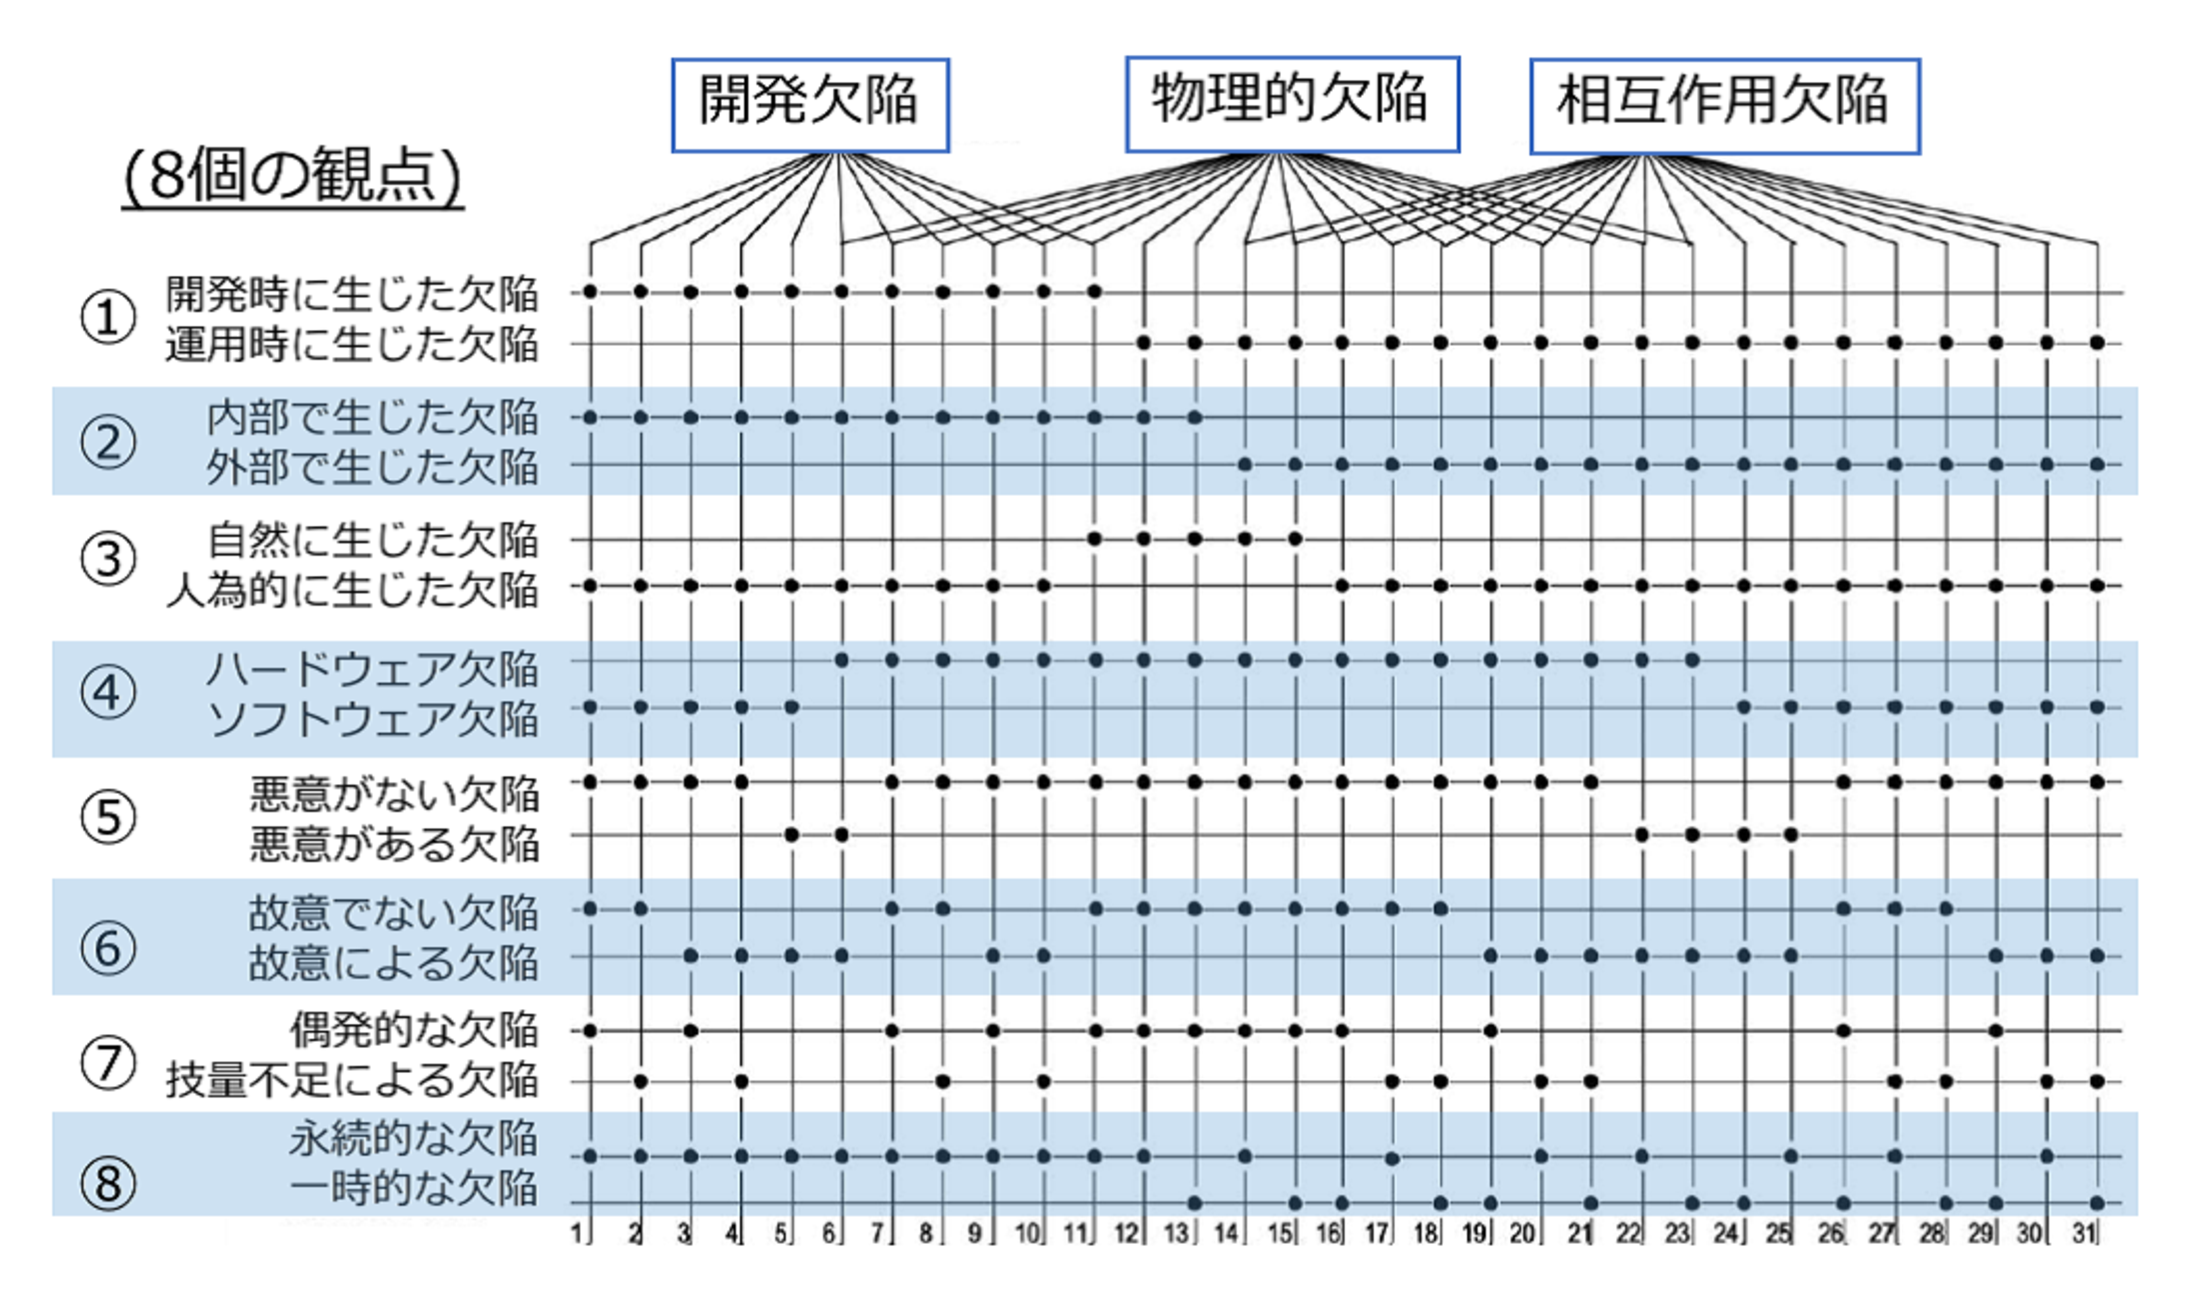
\includegraphics[keepaspectratio, scale=0.2]{classfication.eps}
\caption{���ׂ̕��ތ��ʁi�v�C���j}
\label{���ׂ̕���}
\end{center}
\end{figure}

�{�����ł́A���̕��ނ���\�t�g�E�F�A�Ɋ֌W���A����ɊJ�����ɐ��������̂ɒ��ڂ����B
���̌��ʂR�P�ʂ�̕��ނ��A�}\ref{���ׂ̕���}�Ɏ����P�`�T�Ԃ܂ł̂T�ʂ�ƂȂ����B
����ɁA�h���ӂ����錇�ׁh�͑��݂��Ȃ����̂Ƃ����B
����đΏۂƂ���̂�Intent�̗L���ACapability�̗L����4�‚ł���B


\subsection{�J���v���Z�X}
�{�����ł͉F���q�󌤋��J���@�\�iJAXA�j���񋟂��Ă���A�\�t�g�E�F�A�J���W�����g�p�����B
�����ISO12207�������ɍ��ꂽ���̂ł���B
�\\ref{�Q�‚̃v���Z�X}�Ɏ����悤�Ƀ\�t�g�E�F�A�J���W���͑傫���Q�‚̃v���Z�X���琬�藧���Ă���B

\begin{table}[bp]
\begin{tabular}{|l|l|} \hline
 & �J���v���Z�X \\ \cline{2-1}
�僉�C�t�T�C�N���v���Z�X & �^�p�v���Z�X \\ \cline{2-1}
 & �ێ�v���Z�X \\ \hline

 & �������v���Z�X \\ \cline{2-1}
 & �\���Ǘ��v���Z�X \\ \cline{2-1}
 & �i���ۏ؃v���Z�X \\ \cline{2-1}
�x�����C�t�T�C�N���v���Z�X & ���؃v���Z�X \\ \cline{2-1}
 & �����m�F�v���Z�X \\ \cline{2-1}
 & �������r���[�v���Z�X \\ \cline{2-1}
 & �A�Z�X�����g�v���Z�X \\ \cline{2-1}
 & �������v���Z�X \\ \hline
\end{tabular}
\caption{�僉�C�t�T�C�N���v���Z�X�Ǝx�����C�t�T�C�N���v���Z�X}
\label{�Q�‚̃v���Z�X}
\end{table}

�P�–ڂ��僉�C�t�T�C�N���v���Z�X�ł���A������‚��A�x�����C�t�T�C�N���v���Z�X�ł���B
�僉�C�t�T�C�N���v���Z�X�́A�\�t�g�E�F�A�J���ɒ��ڂ�������Ă���\�t�g�E�F�A���C�t�T�C�N���̃v���Z�X�ł���A�R�‚ɕ������A����ɂ���炪�ׂ����킯���Ă���B
�x�����C�t�T�C�N���́A�僉�C�t�T�C�N���v���Z�X���x����A���̃v���Z�X����Ăт������v���Z�X�ł���A�W�‚ɕ�����ꂨ��A����������l�ɍׂ����������Ă���B
�{�����ł́A�h�v�����s���S�ł��邱�ƂɋN������\�t�g�E�F�A�������炷�h�Ƃ����ړI�����������߁A�\\ref{�J���v���Z�X}�Ɏ����僉�C�t�T�C�N���v���Z�X�̒��̊J���v���Z�X�ɒ��ڂ����B

\begin{table*}[bp]
\begin{tabular}{|l|l|l|} \hline

�t�F�[�Y & �Ή��ԍ� & �ڍׂȓ��e \\ \hline\hline

�v���Z�X�� & 1-1 & �\�t�g�E�F�A�J���v��𗧈Ă��邱�� \\ \cline{2-3}
�J������ & 1-2 & �J���v��̕��͉� \\\hline
�R���s���[�^�V�X�e�� & 2-1& �v���𒊏o���� \\ \cline{2-3}
�v������ & 2-2 & �v���d�l���̍쐬 \\\hline
 & 3-1 & �\������i�ځA��ʂ𖾊m�� \\ \cline{2-3}
 & 3-2 & �e�\���i�ڂɗv�������蓖�Ă� \\ \cline{2-3}
�R���s���[�^�V�X�e�� & 3-3 & �����”\����]�� \\ \cline{2-3}
�����݌v & 3-4 & �݌v�����ƑO������𖾂炩�ɂ��A�]�� \\ \cline{2-3}
 & 3-5 & ��ʂƂ̃g���[�T�r���e�B��]�� \\ \cline{2-3}
 & 3-6 & �C���^�[�t�F�[�X�v���𒊏o \\\hline
 & 4-1 & �\�t�g�E�F�A�v���d�l���̍쐬 \\ \cline{2-3}
 & 4-2 & �•ʂɎ��ʎq��t�^ \\ \cline{2-3}
 & 4-3 & �f�[�^�y�уf�[�^�x�[�X�ɑ΂���d�l���܂߂� \\ \cline{2-3}
 & 4-4 & �ُ팟�m�y�я����Ɋւ���d�l���܂߂� \\ \cline{2-3}
�\�t�g�E�F�A & 4-5 & �C���^�[�t�F�[�X�d�l�Ɋւ��č��ӂ𓾂邱�� \\ \cline{2-3}
�v������ & 4-6 & ��ʂƂ̐������𓾂� \\ \cline{2-3}
 & 4-7 & �����”\���̕]�� \\ \cline{2-3}
 & 4-8 & �����炠����̂��g���Ƃ��͐������Ȃǂ��m�F \\ \cline{2-3}
 & 4-9 & �O������A����𖾊m�� \\ \cline{2-3}
 & 4-10 & ���؉”\����]�� \\ \cline{2-3}
 & 4-11 & �����v��”\����]�� \\ \cline{2-3}
 & 4-12 & �‹���HW�̉e��������ꍇ�m�F�̕]�� \\\hline

\end{tabular}

\caption{�ڍׂȊJ���v���Z�X�i���e�v�ύX�j}
\label{�J���v���Z�X}
\end{table*}



\section{データの適用及び結果}
�{�͂ł͖{�����Ŏg�p����JAXA����񋟂��ꂽ���ۂ̕s��f�[�^�ɂ‚��Đ���������ɁC��q����2�‚̎w�W���ǂ̂悤�Ɏg�p�����̂��ɂ‚��Ă��q�ׂ�D

\subsection{�����Ώ�}
\label{sec:used_data}
�{�����ł́CJAXA�ɂĎ��ۂɔ��������P���ȃv���O�����~�X�ȂǂłȂ�48���̕s����̃��|�[�g��ΏۂƂ����D
���̃��|�[�g�ɂ͂ǂ̃v���W�F�N�g�ŋN�������̂Ȃ̂��C�ǂ̂悤�ȕs��ł��������C���̌����͂Ȃɂ������܂Ƃ߂��Ă���D
�܂��C����48���̃f�[�^��1�‚ɂ‚�1�‚̏�Q�������Ă��邪�C��Q1�‚ɂ‚����ׂ�1�‚ł���Ƃ͌���Ȃ��D

\subsection{���ގ菇}
\label{sec:how_to_class}
�{�����ł͕s��f�[�^�����ׂ̎�ނɂ�蕪�ނ��s�����゠�ƂɊJ���v���Z�X�ɂ�镪�ނ��s�����D
�ڍׂȎ菇�ɂ‚��āC�ȉ��Ɏ����D
\begin{description}
\item[�菇1] �s��i��Q�j1��1�‚ɑ΂��āC���̌����ƂȂ��Ă��錇�ׂ����ł��邩�𖾊m�ɂ���
\item[�菇2] ���m�ɂȂ������ׂɑ΂��āC���ו��ނ̂ǂ�ɊY������̂��𒲂ׁC���x�����O���s����
\item[�菇3] ���x�����O���ꂽ���ׂɑ΂��āC���ꂪ�ǂ̃v���Z�X�Ŕ��������ׂ��ł����������m�F���C�}�b�s���O���s����
\item[�菇4] �}�b�s���O���ꂽ�f�[�^���W�v�C���͂�����
\end{description}
�Ȃ��C����͂��ׂđ�꒘�҂����Ƃōs�������̂ł���D

\subsection{��������}
\label{�W�v}
�s��f�[�^�̕��͂̌��ʁC\ref{sec:used_data}�߂ŏq�ׂ�48���̏�Q����v110���̌��ׂ����o�����D
�����̌��ׂɂ���Q�������N�����ꂽ���̂����邽�߁C���ׂ̐��͏�Q�̐���葽���l�ƂȂ��Ă���D
�܂��C���ʂ������ׂ�\ref{sec:faults}�߂ŏq�ׂ�����1�`4�̂ǂ�ɓ��Ă͂܂邩���꒘�҂��m�F���C���ނ������ʂ�\\ref{�ڍ�}�Ɏ����D
���̕\�ł́C�s�����ɑ΂��ĕ���1�`4�ɊY��������̂������‚������̂��������Ă���D
���̃f�[�^���W�v�����Ƃ���C\ref{sec:faults}�߂ŏq�ׂ�����1��31���C����2��22���C����3��13���C����4��44���ł������D
��L�̌��ʂ�茇�ׂ��ǂ̃v���Z�X�Ŕ������ׂ��ł������̂����m�F���}�b�s���O���s�����D
�}�b�s���O�̌��ʁC1�‚̌��ׂɂ‚��C�����̃v���Z�X�Ō��‚���ׂ����������̂����݂��Ă��邱�Ƃ����������D
����ɁC�v���Z�X����ɕ��ނ������ʂ𕪗�1�`4�ɑ΂��Ă��ꂼ��W�v���C�O���t�����s�����Ƃł��ꂼ��̓����𔭌������D
���̌��ʂɂ‚���\ref{�l�@}�͂ŏq�ׂ�D

\begin{table*}[t]
\caption{��Q�ɑ΂��錇�ׂ̕���}
\label{�ڍ�}
\hbox to\hsize{\hfil
\begin{tabular}{|c|c|c|c|c||c|c|c|c|c||c|c|c|c|c|} \hline
�s����� & \multicolumn{4}{c||}{���ׂ̕���} & �s����� & \multicolumn{4}{c||}{���ׂ̕���} & �s����� & \multicolumn{4}{c|}{���ׂ̕���} \\\cline{2-5}\cline{7-10}\cline{12-15}
 & ����1 & ����2 & ����3 & ����4 &  & ����1 & ����2 & ����3 & ����4 &  & ����1 & ����2 & ����3 & ����4 \\\hline\hline
1 &  & 1 &  & 1 & 17 &  & 1 &  & 1 & 33 & 1 & 1 &  & 2 \\\hline
2 & 1 & 1 &  &  & 18 &  &  &  & 1 & 34 & 1 &  &  & 2 \\\hline
3 & 1 &  &  &  & 19 &  &  & 1 & 1 & 35 & 1 & 1 &  & 1 \\\hline
4 &  &  &  & 1 & 20 & 1 &  &  & 1 & 36 &  &  &  & 1 \\\hline
5 & 1 &  & 1 & 1 & 21 & 1 & 1 & 1 &  & 37 &  & 1 &  & 2 \\\hline
6 & 1 &  &  & 2 & 22 &  & 1 &  &  & 38 &  & 2 & 1 &  \\\hline
7 & 1 &  &  & 1 & 23 &  & 1 &  &  & 39 &  &  & 1 & 2 \\\hline
8 & 1 &  &  & 1 & 24 &  & 1 &  &  & 40 & 1 &  &  &  \\\hline
9 & 1 &  &  & 1 & 25 & 1 &  &  &  & 41 &  & 1 &  &  \\\hline
10 & 1 &  &  & 1 & 26 & 1 & 1 &  & 1 & 42 &  & 1 &  & 2 \\\hline
11 & 1 &  &  & 1 & 27 & 2 & 1 & 2 & 1 & 43 &  & 1 & 1 &  \\\hline
12 &  &  &  & 1 & 28 & 1 &  & 1 & 3 & 44 &  & 1 & 1 &  \\\hline
13 &  &  &  & 1 & 29 & 2 & 1 &  & 3 & 45 &  &  &  & 1 \\\hline
14 & 1 &  &  &  & 30 & 2 & 2 & 1 &  & 46 & 1 &  &  &  \\\hline
15 & 1 &  &  & 2 & 31 &  & 1 &  &  & 47 &  &  & 1 & 1 \\\hline
16 & 3 &  & 1 & 2 & 32 & 1 &  &  & 1 & 48 &  &  &  & 1 \\\hline
\end{tabular}\hfil}
\end{table*}



\begin{comment}
\begin{figure*}
\begin{center}
\includegraphics[keepaspectratio, scale=0.2]{process.eps}
\caption{�v���Z�X�ɂ�镪��}
\label{�v���Z�X�ɂ�镪��}
\end{center}
\end{figure*}
\end{comment}




\section{考察}
�{�͂ł́AJAXA�̃f�[�^�𕪐͂������ʂɂ‚��čl�@���s���B
\subsection{�ςݏグ�O���t�ɂ‚���}
�}\ref{�ςݏグ�O���t}�̃O���t�͉����ɕ\\ref{�J���v���Z�X}�ɋL�ڂ��Ă���JAXA���g�p���Ă���\�t�g�E�F�A�J���W���̃v���Z�X�ɑΉ�����ԍ��ł���B
�܂��c���͕s��̌����ƂȂ��Ă���A�F�����ׂ̕��އ@�A�I�����W�F�����ׂ̕��އA�A�D�F�����ׂ̕��އB�A���F�����ׂ̕��އC�ƂȂ��Ă���B

���̃O���t�Œ��ڂ��ׂ����͍��v�l�������A�v���Z�X4.9��v���Z�X4.1�ł���B
�v���Z�X4.9�Ƃ̓\�t�g�E�F�A�v�����̓t�F�[�Y�̑O������E���񎖍��̒��o�ł���B
�����̋��ʂ��邱�ƂƂ��āA�\�t�g�E�F�A�ȊO�̕����ł̖��m��v�f�ɑ傫�����E�����Ƃ���ł���B
���Ȃ킿�A���̃n�[�h�E�F�A��A�‹��Ȃǂ̉e���ōׂ������߂��ꂸ�ɑ����̌��ׂ����o���ꂽ�ƍl���炦��B
���̎��������������Ƃ������悤�ɁA�v���Z�X4.12��HW��‹���]�����鍀�ڂ̌��ׂ������l�ƂȂ��Ă���B
�܂��A�����ŘR�ꂽ�Ƃ��Ă��A�e�X�g�ŃJ�o�[�ł���΂悢�B
�������A4.11�����̌v��”\���̕]���̒l�������A�s��Ƃ��Č��o�ł��Ȃ����̂������Ȃ��Ă���ƍl������B

\begin{figure*}
\begin{center}
\includegraphics[keepaspectratio, scale=0.2]{add.eps}
\caption{�ςݏグ�O���t}
\label{�ςݏグ�O���t}
\end{center}
\end{figure*}

\subsection{�@+�A�ɂ‚��āi�^�C�g���v�ύX�j}
�}\ref{�P+�Q}�̃O���t�͉����ɕ\\ref{�P+�Q}�ɋL�ڂ��Ă���JAXA���g�p���Ă���\�t�g�E�F�A�J���W���̃v���Z�X�ɑΉ�����ԍ��ł���B
�܂��c���͌��ׂ̐��Ő��K���������̂ƂȂ��Ă���B
�F�͌��ׂ̕��އ@�ƇA�𑫂������̂ƂȂ��Ă���A�I�����W�F�����ׂ̕��ނ̇B�ƇC�𑫂������̂ƂȂ��Ă���B
���Ȃ킿�ADellberate fault��Non-Dellberate fault�ɂ����Ăǂ̂悤�ȍ�������̂������̃O���t���猩���Ă���B

���̃O���t�Œ��ڂ��ׂ����͐F�ƃI�����W�F�̍����傫���Ƃ���ł���B
���Ȃ킿�A�v���Z�X4.6�ł���B
���̍��ڂ͏�ʂƂ̐��������m�F����t�F�[�Y�ł���B
�‚̒l���������Ƃ���A��������ƍl������łȂ��ԈႢ���N���Ă��邱�Ƃ��킩��B
���̗��R�Ƃ��āA�m�F���ׂ���ʂ̐��ʕ����Ȃɂł��邩���l�������ɁA�v���Z�X4.1�̐��ʕ������Ƃ��Ă����邱�Ƃ��ł���B
���̃t�F�[�Y�͕s����������Ƃ͐�قǎ������B
���Ȃ킿�A���S�łȂ��������ʕ��ɑ΂��ă`�F�b�N�������ƂɂȂ�A���ʂƂ��Ă��̃t�F�[�Y�̐F�̍��ڂ��I�����W�ɔ�׍��������ł������ƍl������B

\begin{figure*}
\begin{center}
\includegraphics[keepaspectratio, scale=0.2]{12.eps}
\caption{�@+�A�ƇB+�C�̔�r}
\label{�P+�Q}
\end{center}
\end{figure*}

\subsection{�@+�B�ɂ‚��āi�^�C�g���v�ύX�j}
�}\ref{�P+�R}�̃O���t�͉����ɕ\\ref{�P+�R}�ɋL�ڂ��Ă���JAXA���g�p���Ă���\�t�g�E�F�A�J���W���̃v���Z�X�ɑΉ�����ԍ��ł���B
�܂��c���͌��ׂ̐��Ő��K���������̂ƂȂ��Ă���B
�F�͌��ׂ̕��އ@�ƇB�𑫂������̂ƂȂ��Ă���A�I�����W�F�����ׂ̕��ނ̇A�ƇC�𑫂������̂ƂȂ��Ă���B
���Ȃ킿�AAccidental faults��Incompetence faults�ɂ����Ăǂ̂悤�ȍ�������̂������̃O���t���猩���Ă���B

���̃O���t�ł����ڂ��ׂ����͐F�ƃI�����W�F�̍����傫���Ƃ���ł���4.11�ł���B
������Accidental faults�̒l��Incompetence faults�̒l�ɂ���ׂđ傫�����R�Ƃ��āA�����ł��s�m��v�f�̉e��������A�v�������Ȃ��������Ƃ��N�����̂ł͂Ȃ����ƍl������B

����ŁA����ʂ̃v���Z�X�ł���A1.1�`3.6�ɂ����АF�ɔ�ׂăI�����W�F�̒l���ڗ��Œ��ʂƂȂ��Ă���B
����āA���̕ӂ�ł͋Z�ʂ����Ȃ�d�v�ȃt�@�N�^�[�ƂȂ��Ă���B
����ɁA�����ł̃~�X����X�����Ă��邱�Ƃ����̃O���t����ǂݎ���B
�Ⴆ�΁A�����O������␧��Ɋւ���3.4��4.9�A�v���d�l���Ɋւ���A2.2��4.1�ȂǁA���ɍs���ɂ‚�e�����L�����Ă��邱�Ƃ��ǂݎ���B

\begin{figure*}
\begin{center}
\includegraphics[keepaspectratio, scale=0.2]{13.eps}
\caption{�@+�B�ƇA+�C�̔�r}
\label{�P+�R}
\end{center}
\end{figure*}

\subsection{�e�t�F�[�Y�̊֌W���ɂ‚���}

�\\ref{�e���x}�́A�e�v���Z�X���ǂ̃v���Z�X�ɉe����^���A�ǂ̃v���Z�X����A�e�����󂯂Ă���̂������������̂ł���B
�s������v���Z�X��\���Ă���A�Ή�����ԍ���\�L�����B
���̕\�̐��l�́A�S�͂œ����f�[�^���ڍׂɕ��͂������̂ł���B

\subsubsection{�\�̍쐬���@}
���F�̃Z���ɂ‚��āA���̐��l���ǂ̂悤�ɂ��Čv�Z�������ꂽ���̂ł��邩���������B
��Ƃ��ĉ��F�̌��ɂ‚��Đ���������B
�s��̌����ƂȂ�v���Z�X��4.4�ł�����̂𒊏o�����B
����A4.4�������ł��������͍̂��v�łR�����‚���A���̒l���\�̈�ԉ��̍s�ɋL�q���Ă���B
�܂��P�‚̌��ׂɑ΂��ĕ����̃v���Z�X���Y�����Ă���̂ŁA���̃v���Z�X���J�E���g���A���̒l��4.4�̃v���Z�X���Ŋ���Z�����l�ƂȂ��Ă���B
��������邱�ƂŁA�e�v���Z�X�̈ˑ��֌W�A���Ȃ킿�ǂ̃v���Z�X�ɉe��������̂��A�ǂ̃v���Z�X����e���������Ă���̂������Ă���B

���̐}�ł͍s����������v���Z�X�̏ꍇ�͍��h��ɁA�v�Z�����l��0.5�ȏ�̏ꍇ�͐ԂŐF��h���Ă���B
���Ȃ킿�֌W�����������̂��ԐF�A�֌W�����������̂����F�ƂȂ��Ă���B
�܂��A�����Z�����㑤�ɂ�����̂́A���̃v���Z�X����ʂ̃v���Z�X�ɊY�����邵�A�����ɂ�����̂́A���̃v���Z�X��艺�ʂ̃v���Z�X�ɊY������B

����āA����̗�ł���ƁA�v���Z�X4.4�̓v���Z�X3.2��v���Z�X4.1����̉e���𑽂��󂯂Ă���A�t�ɑ傫���e����^���Ă�����̂͂Ȃ��������ƂɂȂ�B

\subsubsection{�l�@}
���̌��ʂ�蕪���������Ƃ������‚�����B
�܂�1�–ڂƂ��āA����ʂ̍H���ɒ��ڂ���B
�v���Z�X2.1�̓v���Z�X1.1�̉e������ɑ����󂯂Ă���B
�v���Z�X2.2�̓v���Z�X1.1��v���Z�X2.1�̉e�����󂯂Ă���B
�v���Z�X3.1�̓v���Z�X1.1,�v���Z�X2.1,�v���Z�X2.2�̉e�����傫���B
�������猾���邱�Ƃ́A1.1����芮���Ɏd�グ�邱�ƂŁA�v���Z�X2.1,�v���Z�X2.2,�v���Z�X3.1�̕s������ɑ傫�ȉe��������B
���̂�����̃v���Z�X�͏㗬�H���̒��ł����Ȃ��̃v���Z�X�ł���B
�Ȃ̂ŁA�݂��ɉe���������̂͗����ł���B

�Q�–ڂƂ��āA�ł����ׂ̑��������v���Z�X4.9���ւ��Ăł���B
���̃v���Z�X��4.9�ɉe���������炵�Ă���̂̓v���Z�X2.1,�v���Z�X2.2,�v���Z�X3.1,�v���Z�X4.2�ł���B��L�Ŏ������悤�ɁA1.1�̉�����2.1,3.1�̌��ׂ����邱�Ƃ��\�z�����B
�܂��A�v���Z�X3.2��v���Z�X4.2�͉����̉e�����󂯂₷���Ƃ������ʂ͏o�Ă��Ȃ��B
�v���Z�X4.9�����̃v���Z�X����傫�ȉe�����󂯂Ă���킯�ł͂Ȃ��B
�����Ńv���Z�X4.9�����̃v���Z�X����e�����󂯂ɂ����Ɨ��R�Ƃ��āA�O������Ɋւ��鍀�ڂ������ŏ��߂ĂłĂ������߁A���̃t�F�[�Y����ʂ̃t�F�[�Y���疞�ՂȂ��e�����L�����Ă�����̂ƍl������B

����̌��ʂ�葼�̃v���Z�X�ɉe����^����s�|�b�g�ƂȂ��Ă���v���Z�X���������B
����͓���̌�����e�����󂯂Ă��Ȃ����ڂł���B
���Ƃ��Ă͈ȉ��Ɏ������̂�����B
\begin{itemize}
\item �v���Z�X1.1: �\�t�g�E�F�A�J���v��𗧈Ă��邱��
\item �v���Z�X1.2: �J���v��̕��͉�
\item �v���Z�X3.2: �v���d�l���̍쐬
\item �v���Z�X3.3: �����”\����]��
\item �v���Z�X3.5: ��ʂƂ̃g���[�T�r���e�B��]��
\item �v���Z�X3.6: �C���^�[�t�F�[�X�v���𒊏o
\item �v���Z�X4.2: �•ʂɎ��ʎq��t�^
\item �v���Z�X4.3: �f�[�^�y�уf�[�^�x�[�X�ɑ΂���d�l���܂߂�
\end{itemize}
����ŁA�v���Z�X3.3�A�v���Z�X4.2�A�v���Z�X4.3�͍���̃f�[�^�Ɍ��ׂ��Ȃ��܂��͒��������Ȃ��̂ŏ��O�����A�v���Z�X1.1�A�v���Z�X1.2�A�v���Z�X3.2�A�v���Z�X3.5�A�v���Z�X3.6���s�|�b�g�ƂȂ�v���Z�X�ł���ƍl������B


\begin{table*}[bp]
\begin{center}

\begin{tabular}{|l|l|l||l|l|l|l|l|l|l|l|l|l|l|l|l|l|l|l|l|l|l|l|l|} \hline
 \multicolumn{2}{|l|}{�v���Z�X} & 1.1 & 1.2 & 2.1 & 2.2 & 3.1 & 3.2 & 3.3 & 3.4 & 3.5 & 3.6 & 4.1 & 4.2 & 4.3 & 4.4 & 4.5 & 4.6 & 4.7 & 4.8 & 4.9 & 4.10 & 4.11 & 4.12 \\\hline

1.1 & �\�t�g�E�F�A�J���v��𗧈Ă��邱�� & \cellcolor{black}1 & 0.3 & \cellcolor{red}1 & \cellcolor{red}0.5 & 1 & - &  & 0.1 & - & - & 0 & - &  & - & - & - & - & - & 0.1 & 0.1 & - & - \\\hline
1.2 & �J���v��̕��͉� & 0.2 & \cellcolor{black}1 & - & - & - & - &  & - & - & - & - & - &  & - & - & - & - & - & - & - & - & - \\\hline
2.1 & �v���𒊏o���� & \cellcolor{red}0.6 & - & \cellcolor{black}1 & \cellcolor{red}0.5 & 1 & - &  & 0.1 & - & - & 0 & - &  & - & - & - & - & - & 0.1 & 0.1 & - & - \\\hline
2.2 & �v���d�l���̍쐬 & 0.4 & - & \cellcolor{red}0.7 & \cellcolor{black}1 & 1 & - &  & 0.1 & 0.2 & 0.2 & 0.1 & - &  & - & 0.2 & - & - & - & 0.1 & 0.1 & - & - \\\hline
3.1 & �\������i�ځA��ʂ𖾊m�� & 0.4 & - & \cellcolor{red}0.7 & \cellcolor{red}0.5 & \cellcolor{black}1 & - &  & 0.1 & - & - & - & - &  & - & - & - & - & - & 0.1 & 0.1 & - & - \\\hline
3.2 & �e�\���i�ڂɗv�������蓖�Ă� & - & - & - & - & - & \cellcolor{black}1 &  & 0.1 & - & 0.2 & 0.1 & - &  & \cellcolor{red}0.7 & 0.2 & - & - & - & 0 & - & - & - \\\hline
3.3 & �����”\����]�� & - & - & - & - & - & - & \cellcolor{black} & - & - & - & - & - &  & - & - & - & - & - & - & - & - & - \\\hline
3.4 & �݌v�����ƑO������𖾂炩�ɂ��A�]�� & 0.2 & - & 0.3 & 0.3 & \cellcolor{red}0.5 & 0.3 &  & \cellcolor{black}1 & - & - & 0 & - &  & \cellcolor{yellow}0.3 & - & - & - & - & 0.3 & 0.1 & - & 0.1 \\\hline
3.5 & ��ʂƂ̃g���[�T�r���e�B��]�� & - & - & - & 0.3 & - & - &  & - & \cellcolor{black}1 & 0.2 & 0.1 & - &  & - & 0.2 & 0.4 & - & - & 0 & - & - & - \\\hline
3.6 & �C���^�[�t�F�[�X�v���𒊏o & - & - & - & 0.3 & - & 0.3 &  & - & 0.2 & \cellcolor{black}1 & 0.1 & - &  & - & \cellcolor{red}0.8 & - & - & - & - & - & - & 0.1 \\\hline
4.1 & �\�t�g�E�F�A�v���d�l���̍쐬 & 0.2 & - & 0.3 & \cellcolor{red}0.5 & - & \cellcolor{red}0.7 &  & 0.1 & 0.4 & \cellcolor{red}0.6 & \cellcolor{black}1 & - &  & \cellcolor{red}0.7 & \cellcolor{red}0.5 & 0.1 & - & - & 0.2 & - & - & 0.1 \\\hline
4.2 & �•ʂɎ��ʎq��t�^ & - & - & - & - & - & - &  & - & - & - & - & \cellcolor{black}1 &  & - & - & - & - & - & 0 & - & - & - \\\hline
4.3 & �f�[�^�y�уf�[�^�x�[�X�ɑ΂���d�l���܂߂� & - & - & - & - & - & - &  & - & - & - & - & - & \cellcolor{black} & - & - & - & - & - & - & - & - & - \\\hline
4.4 & �ُ팟�m�y�я����Ɋւ���d�l���܂߂� & - & - & - & - & - & \cellcolor{red}0.7 &  & 0.1 & - & - & 0.1 & - &  & \cellcolor{black}1 & - & - & - & - & 0 & - & 0.1 & - \\\hline
4.5 & �C���^�[�t�F�[�X�d�l�Ɋւ��č��ӂ𓾂邱�� & - & - & - & 0.3 & - & 0.3 &  & - & 0.2 & 1 & 0.1 & - &  & - & \cellcolor{black}1 & - & - & 1 & - & - & - & 0.1 \\\hline
4.6 & ��ʂƂ̐������𓾂� & - & - & - & - & - & - &  & - & \cellcolor{red}0.8 & - & 0 & - &  & - & - & \cellcolor{black}1 & - & - & 0.1 & 0.1 & 0.1 & - \\\hline
4.7 & �����”\���̕]�� & - & - & - & - & - & - &  & - & - & - & - & - &  & - & - & - & \cellcolor{black}1 & - & - & - & - & 0.1 \\\hline
4.8 & �����炠����̂��g���Ƃ��͐������Ȃǂ��m�F & - & - & - & - & - & - &  & - & - & - & - & - &  & - & 0.2 & - & - & \cellcolor{black}1 & - & - & - & - \\\hline
4.9 & �O������A����𖾊m�� & 0.4 & - & \cellcolor{red}0.7 & \cellcolor{red}0.5 & \cellcolor{red}1 & 0.3 &  & \cellcolor{red}1 & 0.2 & - & 0.2 & \cellcolor{red}1 &  & 0.3 & - & 0.2 & - & - & \cellcolor{black}1 & 0.1 & - & 0.3 \\\hline
4.1 & ���؉”\����]�� & 0.2 & - & 0.3 & 0.3 & \cellcolor{red}0.5 & - &  & 0.1 & - & - & - & - &  & - & - & 0.1 & - & - & 0 & \cellcolor{black}1 & \cellcolor{red}0.6 & 0.3 \\\hline
4.11 & �����v��”\����]�� & - & - & - & - & - & - &  & - & - & - & - & - &  & 0.3 & - & 0.1 & - & - & - & \cellcolor{red}0.9 & \cellcolor{black}1 & 0.4 \\\hline
4.12 & �‹���HW�̉e��������ꍇ�m�F�̕]�� & - & - & - & - & - & - &  & 0.1 & - & 0.2 & 0 & - &  & - & 0.2 & - & 0.3 & - & 0.1 & 0.3 & 0.3 & \cellcolor{black}1 \\\hline
\multicolumn{2}{|l|}{�ΏۂƂȂ�t�F�[�Y�̕s��f�[�^�̌�} & 5  & 4  & 3  & 4  & 2  & 3  & 0  & 8  & 5  & 5  & 21  & 1  & 0  & 3  & 6  & 9  & 3  & 1  & 28  & 10  & 16  & 12  \\\hline



\end{tabular}
\end{center}
\caption{�e�v���Z�X�ւ̉e���x}
\label{�e���x}
\end{table*}



\begin{comment}
\begin{table*}[bp]
\begin{center}
\begin{tabular}{|l|l|l|l|l|l|l|l|l|l|l|l|l|l|l|l|l|l|l|l|l|l|l|l|} \hline
1.1 & �\�t�g�E�F�A�J���v��𗧈Ă��邱�� & \cellcolor{black}1 & 0.3 & 1 & 0.5 & 1 & - &  & 0.1 & - & - & 0 & - &  & - & - & - & - & - & 0.1 & 0.1 & - & - \\\hline
1.2 & �J���v��̕��͉� & 0.2 & \cellcolor{black}1 & - & - & - & - &  & - & - & - & - & - &  & - & - & - & - & - & - & - & - & - \\\hline
2.1 & �v���𒊏o���� & 0.6 & - & \cellcolor{black}1 & 0.5 & 1 & - &  & 0.1 & - & - & 0 & - &  & - & - & - & - & - & 0.1 & 0.1 & - & - \\\hline
2.2 & �v���d�l���̍쐬 & 0.4 & - & 0.7 & \cellcolor{black}1 & 1 & - &  & 0.1 & 0.2 & 0.2 & 0.1 & - &  & - & 0.2 & - & - & - & 0.1 & 0.1 & - & - \\\hline
3.1 & �\������i�ځA��ʂ𖾊m�� & 0.4 & - & 0.7 & 0.5 & \cellcolor{black}1 & - &  & 0.1 & - & - & - & - &  & - & - & - & - & - & 0.1 & 0.1 & - & - \\\hline
3.2 & �e�\���i�ڂɗv�������蓖�Ă� & - & - & - & - & - & \cellcolor{black}1 &  & 0.1 & - & 0.2 & 0.1 & - &  & 0.7 & 0.2 & - & - & - & 0 & - & - & - \\\hline
3.3 & �����”\����]�� & - & - & - & - & - & - & \cellcolor{black} & - & - & - & - & - &  & - & - & - & - & - & - & - & - & - \\\hline
3.4 & �݌v�����ƑO������𖾂炩�ɂ��A�]�� & 0.2 & - & 0.3 & 0.3 & 0.5 & 0.3 &  & \cellcolor{black}1 & - & - & 0 & - &  & 0.3 & - & - & - & - & 0.3 & 0.1 & - & 0.1 \\\hline
3.5 & ��ʂƂ̃g���[�T�r���e�B��]�� & - & - & - & 0.3 & - & - &  & - & \cellcolor{black}1 & 0.2 & 0.1 & - &  & - & 0.2 & 0.4 & - & - & 0 & - & - & - \\\hline
3.6 & �C���^�[�t�F�[�X�v���𒊏o & - & - & - & 0.3 & - & 0.3 &  & - & 0.2 & \cellcolor{black}1 & 0.1 & - &  & - & 0.8 & - & - & - & - & - & - & 0.1 \\\hline
4.1 & �\�t�g�E�F�A�v���d�l���̍쐬 & 0.2 & - & 0.3 & 0.5 & - & 0.7 &  & 0.1 & 0.4 & 0.6 & \cellcolor{black}1 & - &  & 0.7 & 0.5 & 0.1 & - & - & 0.2 & - & - & 0.1 \\\hline
4.2 & �•ʂɎ��ʎq��t�^ & - & - & - & - & - & - &  & - & - & - & - & \cellcolor{black}1 &  & - & - & - & - & - & 0 & - & - & - \\\hline
4.3 & �f�[�^�y�уf�[�^�x�[�X�ɑ΂���d�l���܂߂� & - & - & - & - & - & - &  & - & - & - & - & - & \cellcolor{black} & - & - & - & - & - & - & - & - & - \\\hline
4.4 & �ُ팟�m�y�я����Ɋւ���d�l���܂߂� & - & - & - & - & - & 0.7 &  & 0.1 & - & - & 0.1 & - &  & \cellcolor{black}1 & - & - & - & - & 0 & - & 0.1 & - \\\hline
4.5 & �C���^�[�t�F�[�X�d�l�Ɋւ��č��ӂ𓾂邱�� & - & - & - & 0.3 & - & 0.3 &  & - & 0.2 & 1 & 0.1 & - &  & - & \cellcolor{black}1 & - & - & 1 & - & - & - & 0.1 \\\hline
4.6 & ��ʂƂ̐������𓾂� & - & - & - & - & - & - &  & - & 0.8 & - & 0 & - &  & - & - & \cellcolor{black}1 & - & - & 0.1 & 0.1 & 0.1 & - \\\hline
4.7 & �����”\���̕]�� & - & - & - & - & - & - &  & - & - & - & - & - &  & - & - & - & \cellcolor{black}1 & - & - & - & - & 0.1 \\\hline
4.8 & �����炠����̂��g���Ƃ��͐������Ȃǂ��m�F & - & - & - & - & - & - &  & - & - & - & - & - &  & - & 0.2 & - & - & \cellcolor{black}1 & - & - & - & - \\\hline
4.9 & �O������A����𖾊m�� & 0.4 & - & 0.7 & 0.5 & 1 & 0.3 &  & 1 & 0.2 & - & 0.2 & 1 &  & 0.3 & - & 0.2 & - & - & \cellcolor{black}1 & 0.1 & - & 0.3 \\\hline
4.1 & ���؉”\����]�� & 0.2 & - & 0.3 & 0.3 & 0.5 & - &  & 0.1 & - & - & - & - &  & - & - & 0.1 & - & - & 0 & \cellcolor{black}1 & 0.6 & 0.3 \\\hline
4.11 & �����v��”\����]�� & - & - & - & - & - & - &  & - & - & - & - & - &  & 0.3 & - & 0.1 & - & - & - & 0.9 & \cellcolor{black}1 & 0.4 \\\hline
4.12 & �‹���HW�̉e��������ꍇ�m�F�̕]�� & - & - & - & - & - & - &  & 0.1 & - & 0.2 & 0 & - &  & - & 0.2 & - & 0.3 & - & 0.1 & 0.3 & 0.3 & \cellcolor{black}1 \\\hline
\multicolumn{2}{|l|}{�s��f�[�^�̌�} & 5  & 4  & 3  & 4  & 2  & 3  & 0  & 8  & 5  & 5  & 21  & 1  & 0  & 3  & 6  & 9  & 3  & 1  & 28  & 10  & 16  & 12  \\\hline
\end{tabular}
\end{center}
\caption{�e�v���Z�X�ւ̉e���x}
\label{eikyoudo }
\end{table*}
�[�~�̃��X�g�̌��ʂ̕����A�^�C�ŕ��͂������ʂ̍l�@�Ȃǂ��ڂ���
\end{comment}

\section{まとめ}
�p�������ނ́C�ÓI�Ȍ��ׂɂ�镪�ޖ@�ƁC���I�ȊJ���v���Z�X�����킹�����̂ł���C�v�����s���S�ł��邱�ƂɋN������\�t�g�E�F�A���̕��ޖ@��񎦂��Ă���D
�s��f�[�^���炱�̕��ނ��s�����ƂŁC�s��̌X����m�邱�Ƃ��ł��C�v���Z�X�Ƃ��Ăǂ��ɗ͂�����ׂ��ł��邩�������Ă���D
����ŁC�K�p�����g�D�ɂ�����v���Z�X�Ԃ̉e���x���m�邱�Ƃ��ł��C�����悭�΍���u���邱�Ƃ����҂����D

����CJAXA�̖�50���̕s��f�[�^�����Ɍ��ׂ̌X����v���Z�X�Ԃ̉e���ɂ‚��ĕ��͂��s�������C���̑g�D�ł��g�p���Ă���v���Z�X�𓖂Ă͂߂邱�ƂŁC���l�̕��͂��s�����Ƃ��”\�ł���C���ׂ̌X����C�v���Z�X�Ԃ̉e���ɂ‚��ċc�_���ł���ƍl���Ă���D

�{�����ł́C�s��̌X����v���Z�X�Ԃ̉e����m�邱�Ƃ͂ł������C����̉ۑ�Ƃ��Ă����΂���΍���@�̒񎦁E��������������D




\ack %% 謝辞

\bibliographystyle{sieicej}
\bibliography{ref}
%\begin{thebibliography}{99}% 文献数が10未満の時 {9}
%\bibitem{}




%\end{thebibliography}

\appendix
�\\ref{���ׂ̐�}�̏ڍׂȃf�[�^�ł���B
\begin{table}[bp]
\begin{tabular}{|c|c|c|c|c||c|c|c|c|c||c|c|c|c|c|} \hline
�s����� & \multicolumn{4}{c||}{���ׂ̕���} & �s����� & \multicolumn{4}{c||}{���ׂ̕���} & �s����� & \multicolumn{4}{c|}{���ׂ̕���} \\\cline{2-5}\cline{7-10}\cline{12-15}
 & �@ & �A & �B & �C &  & �@ & �A & �B & �C &  & �@ & �A & �B & �C \\\hline\hline
1 &  & 1 &  & 1 & 17 &  & 1 &  & 1 & 33 & 1 & 1 &  & 2 \\\hline
2 & 1 & 1 &  &  & 18 &  &  &  & 1 & 34 & 1 &  &  & 2 \\\hline
3 & 1 &  &  &  & 19 &  &  & 1 & 1 & 35 & 1 & 1 &  & 1 \\\hline
4 &  &  &  & 1 & 20 & 1 &  &  & 1 & 36 &  &  &  & 1 \\\hline
5 & 1 &  & 1 & 1 & 21 & 1 & 1 & 1 &  & 37 &  & 1 &  & 2 \\\hline
6 & 1 &  &  & 2 & 22 &  & 1 &  &  & 38 &  & 2 & 1 &  \\\hline
7 & 1 &  &  & 1 & 23 &  & 1 &  &  & 39 &  &  & 1 & 2 \\\hline
8 & 1 &  &  & 1 & 24 &  & 1 &  &  & 40 & 1 &  &  &  \\\hline
9 & 1 &  &  & 1 & 25 & 1 &  &  &  & 41 &  & 1 &  &  \\\hline
10 & 1 &  &  & 1 & 26 & 1 & 1 &  & 1 & 42 &  & 1 &  & 2 \\\hline
11 & 1 &  &  & 1 & 27 & 2 & 1 & 2 & 1 & 43 &  & 1 & 1 &  \\\hline
12 &  &  &  & 1 & 28 & 1 &  & 1 & 3 & 44 &  & 1 & 1 &  \\\hline
13 &  &  &  & 1 & 29 & 2 & 1 &  & 3 & 45 &  &  &  & 1 \\\hline
14 & 1 &  &  &  & 30 & 2 & 2 & 1 &  & 46 & 1 &  &  &  \\\hline
15 & 1 &  &  & 2 & 31 &  & 1 &  &  & 47 &  &  & 1 & 1 \\\hline
16 & 3 &  & 1 & 2 & 32 & 1 &  &  & 1 & 48 &  &  &  & 1 \\\hline
\end{tabular}
\caption{�ڍׂȌ��ׂɑ΂���s��̐�}
\label{�ڍׂP}
\end{table}

\section{}

\begin{biography}
\profile{}{}{}
%\profile{会員種別}{名前}{紹介文}% 顔写真あり
%\profile*{会員種別}{名前}{紹介文}% 顔写真なし
\end{biography}

\end{document}



%% 2. 「レター」
\documentclass[letter]{ieicej}
%\usepackage[dvips]{graphicx}
%\usepackage[dvipdfmx]{graphicx,xcolor}
\usepackage[T1]{fontenc}
\usepackage{lmodern}
\usepackage{textcomp}
\usepackage{latexsym}
%\usepackage[fleqn]{amsmath}
%\usepackage{amssymb}

\setcounter{page}{1}

\typeofletter{研究速報}
%\typeofletter{紙上討論}
%\typeofletter{問題提起}
%\typeofletter{ショートノート}
\field{}
\jtitle{}
\etitle{}
\authorlist{%
 \authorentry{}{}{}{}\MembershipNumber{}
 %\authorentry{和文著者名}{英文著者名}{会員種別}{所属ラベル}\MembershipNumber{}
 %\authorentry{和文著者名}{英文著者名}{会員種別}{所属ラベル}[現在の所属ラベル]\MembershipNumber{}
}
\affiliate[]{}{}
%\affiliate[所属ラベル]{和文所属}{英文所属}
%\paffiliate[]{}
%\paffiliate[現在の所属ラベル]{和文所属}

\begin{document}
\maketitle
\begin{abstract}
%和文あらまし 120字以内
\end{abstract}
\begin{keyword}
%和文キーワード 4〜5語
\end{keyword}
\begin{eabstract}
%英文アブストラクト 50 words
\end{eabstract}
\begin{ekeyword}
%英文キーワード
\end{ekeyword}

\section{まえがき}


\ack %% 謝辞

%\bibliographystyle{sieicej}
%\bibliography{myrefs}
\begin{thebibliography}{99}% 文献数が10未満の時 {9}
\bibitem{}
\end{thebibliography}

\appendix
\section{}

\end{document}


%% 3. 「レター(C分冊)」
\documentclass[electronicsletter]{ieicej}
%\usepackage[dvips]{graphicx}
%\usepackage[dvipdfmx]{graphicx,xcolor}
\usepackage[T1]{fontenc}
\usepackage{lmodern}
\usepackage{textcomp}
\usepackage{latexsym}
%\usepackage[fleqn]{amsmath}
%\usepackage{amssymb}

\setcounter{page}{1}

\field{}
\jtitle{}
\etitle{}
\authorlist{%
 \authorentry{}{}{}{}\MembershipNumber{}
 %\authorentry{和文著者名}{英文著者名}{会員種別}{所属ラベル}\MembershipNumber{}
 %\authorentry{和文著者名}{英文著者名}{会員種別}{所属ラベル}[現在の所属ラベル]\MembershipNumber{}
}
\affiliate[]{}{}
%\affiliate[所属ラベル]{和文所属}{英文所属}
%\paffiliate[]{}
%\paffiliate[現在の所属ラベル]{和文所属}

\begin{document}
\begin{abstract}
%和文あらまし 120字以内
\end{abstract}
\begin{keyword}
%和文キーワード 4〜5語
\end{keyword}
\begin{eabstract}
%英文アブストラクト 50 words
\end{eabstract}
\begin{ekeyword}
%英文キーワード
\end{ekeyword}
\maketitle

\section{まえがき}


\ack %% 謝辞

%\bibliographystyle{sieicej}
%\bibliography{myrefs}
\begin{thebibliography}{99}% 文献数が 10 未満の時 {9}
\bibitem{}
\end{thebibliography}

\appendix
\section{}

\end{document}



%% 4. 「技術研究報告」
\documentclass[technicalreport]{ieicej}
%\usepackage[dvips]{graphicx}
%\usepackage[dvipdfmx]{graphicx,xcolor}
\usepackage[T1]{fontenc}
\usepackage{lmodern}
\usepackage{textcomp}
\usepackage{latexsym}
%\usepackage[fleqn]{amsmath}
%\usepackage{amssymb}

\jtitle{}
\jsubtitle{}
\etitle{}
\esubtitle{}
\authorlist{%
 \authorentry[]{}{}{}
% \authorentry[メールアドレス]{和文著者名}{英文著者名}{所属ラベル}
}
\affiliate[]{}{}
%\affiliate[所属ラベル]{和文勤務先\\ 連絡先住所}{英文勤務先\\ 英文連絡先住所}

\begin{document}
\begin{jabstract}
%和文あらまし
\end{jabstract}
\begin{jkeyword}
%和文キーワード
\end{jkeyword}
\begin{eabstract}
%英文アブストラクト
\end{eabstract}
\begin{ekeyword}
%英文キーワード
\end{ekeyword}
\maketitle

\section{はじめに}


%\bibliographystyle{sieicej}
%\bibliography{myrefs}
%\begin{thebibliography}{99}% 文献数が10未満の時 {9}
%\bibitem{}
\end{thebibliography}

\end{document}
